\newsection
\section{Техническое задание}
\subsection{Основание для разработки}

Основанием для разработки данного приложения является задание на выпускную квалификационную работу бакалавра «Программно-информационная система доя организации работы медицинской лаборатории» согласно приказу №1507-с от 7 апреля 2023 г.

\subsection{Цель и назначение разработки}

Основная цель веб-сайта медицинской лаборатории - предоставить четкую и подробную информацию о предлагаемых услугах. Сюда входит информация о проводимых тестах, диагностических услугах и доступных методах лечения. Кроме того, на сайте может быть представлена информация о врачах и персонале медицинской лаборатории.

Основной целью данной выпускной квалификационной работы является разработка и внедрение веб-сайта для управления регистрационными данными и результатами медицинской лаборатории "KLLABORATORY".

При разработке веб-сайта для медицинской лаборатории были учтены некоторые ключевые аспекты. Ниже перечислены некоторые из них:

\begin{enumerate}
	\item Определить потребности медицинской лаборатории: мы проанализировали, какую информацию и услуги лаборатория хочет предоставить пользователям на своем сайте.
	\item Определить удобный и понятный для пользователя дизайн: веб-сайт должен быть простым в навигации для пользователей и предоставлять информацию в ясной и организованной форме.
	\item Информационная безопасность: необходимо обеспечить безопасность и конфиденциальность информации, предоставляемой пациентами.
	\item Актуальная информация: веб-сайт должен содержать актуальную и точную информацию о лаборатории, предлагаемых услугах и результатах анализов.
	\item Интеграция с технологиями: следует рассмотреть возможность интеграции передовых технологий, чтобы сделать работу пользователя более приятной и эффективной, например, онлайн-платформа для записи информации о пациентах, врачах и специальностях для доставки результатов анализов.
	\item Фокус на пользовательском опыте: веб-сайт должен быть разработан с учетом пользовательского опыта и того, как он может облегчить доступ к информации и услугам, предлагаемым медицинской лабораторией.   
\end{enumerate}

Использование веб-сайта в медицинской лаборатории окажет значительное влияние на обслуживание пациентов и эффективность работы лаборатории. Веб-сайт можно использовать для информирования клиницистов о процедурах, проводимых с пациентом, о показаниях, которым он должен следовать перед прохождением лабораторного обследования, и о результатах проведенных анализов. Это может помочь врачам лучше понять состояние здоровья пациента и принять решение о лечении.

Кроме того, использование веб-сайта может повысить внутреннюю эффективность медицинской лаборатории за счет организации и составления расписания тестирования пациентов. Это может сократить время ожидания для пациентов, минимизировать человеческие ошибки и повысить общую эффективность работы лаборатории.

Однако важно отметить, что правильное оформление и обслуживание веб-сайта имеет решающее значение для обеспечения его соответствия требованиям конфиденциальности и безопасности медицинской информации. Кроме того, веб-сайт должен регулярно обновляться, чтобы обеспечить адекватность и точность представленной информации.

С помощью внедрения веб-сайта планируется устранить существующие недостатки в работе медицинской лаборатории. Исходя из этого, предлагается рассмотреть основную цель в контексте двух групп подцелей.

Задачами данной разработки являются:
\begin{itemize}
\item создание информативных разделов на сайте;
\item внедрение регистрационных форм;
\item внедрение динамической таблицы пациентов;
\item создание пользователей и паролей врачей.
\end{itemize}

\subsection{Требования пользователя к интерфейсу web-сайта}

Интерфейс сайта медицинской лаборатории интуитивно понятен и удобен для пользователя. Важно, чтобы врачи могли быстро найти необходимую информацию и чтобы навигация по сайту была плавной. Сайт предоставляет подробную информацию о предлагаемых услугах и должен легко обновляться новой информацией. Сайт должен быть визуально привлекательным и использовать графику и другие визуальные элементы для предоставления дополнительной информации.

Разработанный веб-сайт не будет предоставлять информацию о местонахождении медицинской лаборатории или расписании приемов, поскольку он предназначен только для внутреннего пользования, доступ к нему будут иметь только уполномоченные врачи, которые будут отвечать за регистрацию и обновление информации о новых пациентах.

Важно, чтобы врачи, использующие веб-сайт медицинской лаборатории, имели интуитивно понятный пользовательский опыт. Ниже приведены некоторые требования, которые могут принести пользу врачам, использующим веб-сайт медицинской лаборатории:

\begin{enumerate}
	\item Простой и интуитивно понятный дизайн: веб-сайт должен быть простым в навигации и использовании, с чистым и функциональным дизайном. Врачи могут быстро и эффективно найти то, что им нужно.
	\item Доступность: сайт легко доступен для врачей с разным уровнем владения компьютером и разных специальностей.
	\item Полная и актуальная информация: врачи имеют доступ к полной и актуальной информации о процессах, методах лечения и результатах анализов, проведенных в медицинской лаборатории.
	\item Безопасная платформа: Веб-платформа разработана для защиты конфиденциальной медицинской информации пациентов. Соответствует установленным нормативным требованиям и требованиям безопасности.
\end{enumerate}

Сайт должен включать в себя:
\begin{itemize}
    \item навигацию по разделам;
    \item авторизацию;
    \item доступ администратора и редактора к формам.
\end{itemize}

Для взаимодействия врача или медсестры с сайтом был согласован удобный интерфейс для эффективного и простого использования. На сайте будет навигационное меню, расположенное в левой части экрана, где можно выбрать специальности и зарегистрировать врачей и пациентов. В нижней части навигационного меню находится кнопка для закрытия текущей сессии, в которой зарегистрирован врач. В верхней части навигационного меню расположено изображение логотипа медицинской лаборатории.

Композиция шаблона сайта представлена на рисунке ~\ref{img:pagp}.

\begin{figure}
\center{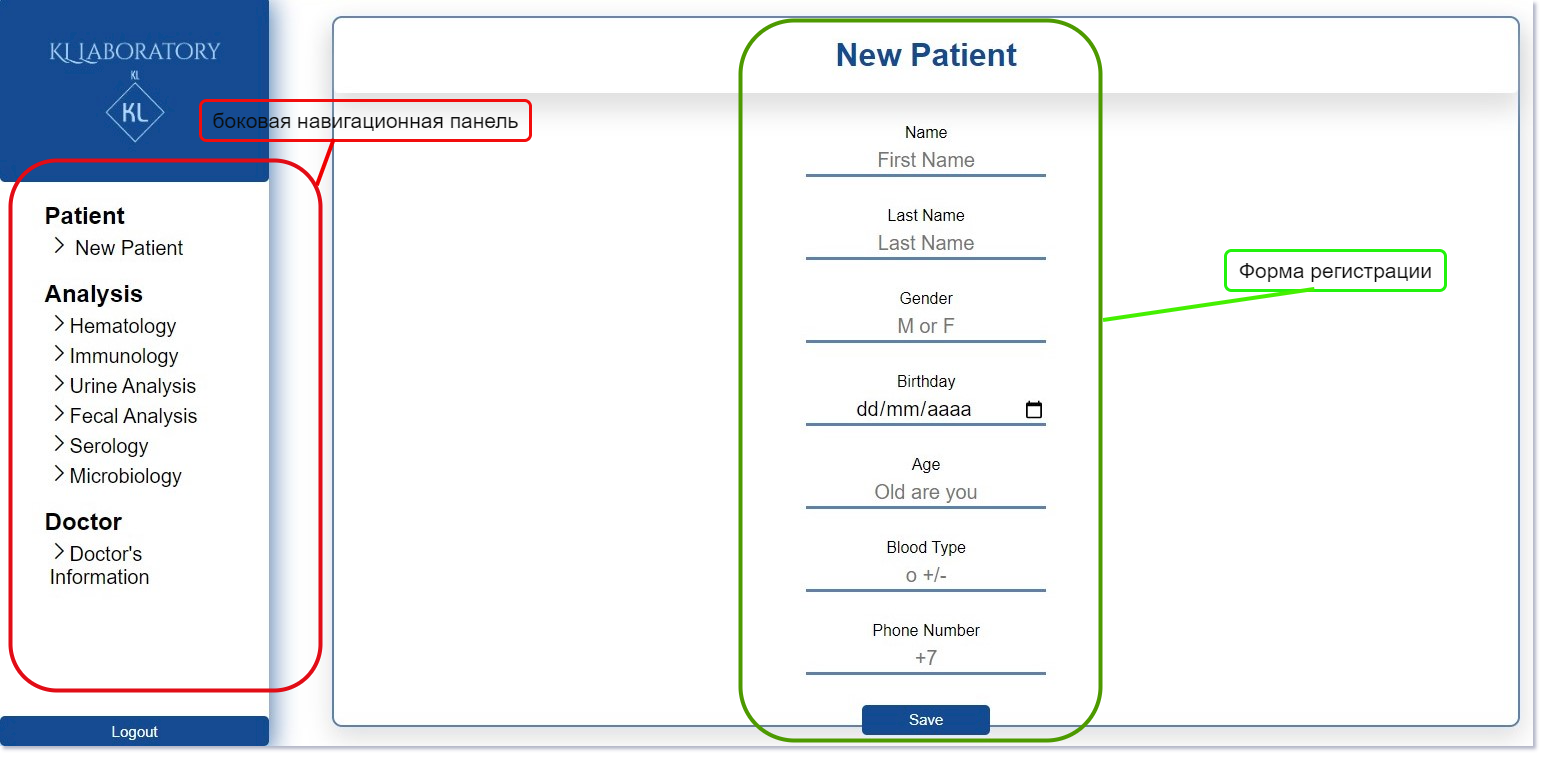
\includegraphics[width=1\linewidth]{pag1}}
\caption{Композиция шаблона сайта}
\label{img:pagp}
\end{figure}

\subsubsection{Исследование предметной области}

Веб-страница в медицинской лаборатории оказывает большую помощь и пользу врачам и персоналу клиники, поскольку служит полезным инструментом для всех процессов, которые они хотят выполнить.
Пользователь должен быть обученным врачом или медсестрой, чтобы правильно ввести данные по каждой процедуре на каждой специализированной форме.
Поля для ввода информации имеют свою собственную связь с базой данных.
В меню врач может перемещаться и выбирать нужную специальность для соответствующей записи. 
Сайт имеет четыре основные функции: сохранение формы, загрузка базы данных пациентов, начало и выход. 

\subsection{Требования к функциональным характеристикам}

\subsubsection{Прецеденты}

Разрабатываемая веб-система предназначена для облегчения управления пациентами и врачами в медицинской лаборатории. На основе изучения конкретного случая было выявлено несколько прецедентов, которые были реализованы на сайте.

Первый прецедент, ``Registration New Patient'', позволяет врачам вводить персональные данные пациентов, приходящих в медицинскую лабораторию. Далее, прецедент ``Save Patient'' используется для проверки и сохранения информации, введенной в форму, и сохранения ее в базе данных системы.

После сохранения данных пациента прецедент ``Choose Analysis'' позволяет врачу или медсестре выбрать тест той специальности, которая необходима пациенту. 

Перед ``Enter Hematology results'' врач или медсестра должны записать все проведенные тесты вместе с результатами для соответствующей проверки врачом и после оценки врачом написать лечение пациента в том же отделе ``Hematology''. Далее используется прецедент ``Save form'', нажав кнопку сохранения, система проверит информацию и сохранит ее в таблице ``Hematology'' в базе данных.

Предшествующая форма ``Enter Immunology Results'' позволяет врачу или медсестре ввести информацию для проведения обследования пациента, следуя полям формы ``Immunology'', таким же образом ввести результаты для соответствующей проверки врача и лечения пациента. После этого прецедента используется прецедент ``Save Form'', когда врач или медсестра хочет сохранить записи в форме ``Immunology'' в базе данных системы.

Прецедент ``Enter Analysis Urine Result'' позволяет врачу или медсестре ввести информацию об исследованиях, анализах и результатах, проведенных у пациента, для соответствующего подтверждения врачом и перехода к назначению соответствующего лечения пациенту. Далее, прецедент ``Save form`` позволяет врачу или медсестре сохранить все данные, введенные в форму, в таблице ``Urine'' в базе данных.

Прецедент ``Enter Fecal Analysis Results'' позволяет врачу или медсестре ввести информацию из всех полей формы по специальности ``Fecal Analysis'', т.е. осмотр, анализ и результаты пациента, для оценки врачом и записи истории болезни и лечения пациента. Далее используется прецедент ``Save form'', позволяющий врачу или медсестре сохранить информацию, введенную в форму ``Fecal Analysis'' для записи на вкладке в базе данных системы.

Прецедент ``Enter Serology Results'' позволяет врачу или медсестре ввести информацию об исследованиях, анализах и результатах, проведенных по специальности для пациента, для соответствующей оценки врачом и лечения пациента. После ввода данных команда ``Save form'' позволяет врачу или медсестре сохранить все введенные в форму данные в резервном файле.

Прецедент ``Enter Microbiology Results'' это позволяет врачу или медсестре вводить информацию, которая предоставляется пациенту, заполняя поля формы ``Microbiology'', а также вводить данные результатов для соответствующей проверки врачом.и лечение, которое необходимо провести пациенту. После этого прецедента продолжается прецедент ``Save form'', который используется, когда врач или медсестра хотят сохранить введенные данные в форме ``Microbiology'' в табе, назначенном для специальности в базе данных системы.

Первый прецедент, ``Registration New Doctor'', позволяет врачу или медсестре вводить личную информацию нового врача, который будет работать в медицинской лаборатории, а также имя пользователя и пароль, назначенные для входа в систему веб-сайта. Далее, предыдущее ``Save Doctor'' используется для проверки и сохранения информации, введенной из формы, и сохранения в базе данных системы.

Наконец, прецедентная ``Information'' позволяет врачу или медсестре проверять и анализировать в таблице всю информацию о пациентах, зарегистрированных в медицинской лаборатории.

Таким образом, использование этих прецедентов на веб-сайте медицинской лаборатории позволяет эффективно управлять пациентами, врачами и специалистами, а также предлагает практическое решение для управления информацией, необходимой в медицинской лаборатории.

Диаграмма приоритетов для программной среды изображена на рисунке \ref{img:usua}.

\begin{figure}
	\center{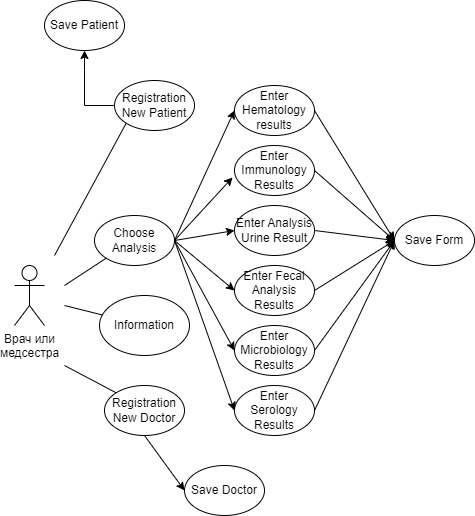
\includegraphics[width=1\linewidth]{diagramauso}}
	\caption{Диаграмма прецедентов}
	\label{img:usua}
\end{figure}

\subsubsection{Сценарии прецедентов программного изделия}

Сценарий для варианта использования "Пользователь и пароль".
Главное действующее лицо: врач или медсестра.
Действующие лица и их требования: врачу или медсестре необходимо будет войти в систему, введя идентификатор пользователя и пароль зарегистрированного врача .
Предварительное условие: наличие подключения к Интернету и должна быть загружена веб-страница медицинской лаборатории.
Последующее условие: После подтверждения врачом идентификатора пользователя и пароля врач или медсестра получат доступ ко всей информации и формам всех специализированных служб, информации о врачах и пациентах медицинской лаборатории.

Основной сценарий успеха:

\begin{enumerate}
	\item Пользователь вводит правильное имя пользователя и пароль.
	\item Пользователь нажимает кнопку ``New Patient''.
	\item Система отображает форму нового пациента.
	\item Пользователь вводит информацию в поля формы.
	\item Пользователь нажимает кнопку ``Save''.
	\item Система записывает всю информацию, введенную в поля формы нового пациента.
	\item Система отображает сообщение об эффективном сохранении.
	\item Пользователь нажимает на меню ``New Doctor''.
	\item Система отображает форму для приема к новому врачу.
	\item Пользователь заполняет поля формы нового врача.
	\item Пользователь нажимает кнопку ``Save''.
	\item Система записывает информацию, внесенную в таблицу врачей, в базу данных.
	\item Система отображает сообщение об эффективности сохранения в системной базе данных.
	\item Пользователь выбирает из меню специальность ``Hematology''.
	\item Система отображает анкету по специальности ``Hematology''.
	\item Пользователь вводит запрашиваемую информацию в специальную форму.
	\item Пользователь нажимает кнопку ``Save''.
	\item Система записывает информацию, внесенную в таблицу ``Hematology'', в базу данных системы.
	\item Система отображает временное сообщение о фактическом сохранении.
	\item Пользователь выбирает из меню специальность ``Immunology''.
	\item Система отображает анкету по специальности ``Immunology''.
	\item Пользователь вводит запрашиваемую информацию в специальную форму.
	\item Пользователь нажимает кнопку ``Save''.
	\item Система записывает информацию, введенную в таблицу ``Immunology'', в базу данных системы.
	\item Система отображает временное сообщение о фактическом сохранении.
	\item Пользователь выбирает из меню специальность ``Urine Analysis''.
	\item Система отображает форму по специальности ``Urine Analysis''.
	\item Пользователь вводит запрашиваемую информацию в специальную форму.
	\item Пользователь нажимает кнопку ``Save''.
	\item Система записывает информацию, введенную в таблицу ``Urine'', в базу данных системы.
	\item Система отображает временное сообщение о фактическом сохранении.
	\item Пользователь выбирает из меню специальность ``Fecal Analysis''.
	\item Система отображает форму по специальности ``Fecal Analysis''.
	\item Пользователь вводит запрашиваемую информацию в специальную форму.
	\item Пользователь нажимает кнопку ``Save''.
	\item Система записывает информацию, введенную в таблицу ``Fecal'', в базу данных системы.
	\item Система отображает временное сообщение о фактическом сохранении.
	\item Пользователь выбирает из меню специальность ``Serology''.
	\item Система отображает анкету по специальности ``Serology''.
	\item Пользователь вводит запрашиваемую информацию в специальную форму.
	\item Пользователь нажимает кнопку ``Save''.
	\item Система записывает информацию, введенную в таблицу ``Serology'', в базу данных системы.
	\item Система отображает временное сообщение о фактическом сохранении.
	\item Пользователь выбирает из меню специальность ``Microbiology''.
	\item Система отображает анкету по специальности ``Microbiology''.
	\item Пользователь вводит запрашиваемую информацию в специальную форму.
	\item Пользователь нажимает кнопку ``Save''.
	\item Система записывает информацию, внесенную в таблицу ``Microbiology'', в базу данных системы.
	\item Система отображает временное сообщение о фактическом сохранении.
	\item Пользователь выбирает из меню специальность ``Information''.
	\item Система отображает таблицу со всей информацией о пациентах, зарегистрированных в медицинской лаборатории.
	\item Пользователь нажимает кнопку выхода.
	\item Вошедший в систему пользователь выходит из системы.
\end{enumerate}

\subsection{Моделирование вариантов использования}

Моделирование сценариев использования - это популярный подход, используемый для понимания функциональных возможностей и требований веб-сайта. В случае медицинской лаборатории варианты использования основаны на потребностях пациентов и лаборатории.

В случае использования веб-сайта медицинской лаборатории врачи должны иметь возможность доступа к подробной информации об услугах, предлагаемых лабораторией, и личной информации о пациентах. Сюда входит информация о проведенных тестах, диагностических услугах и доступных методах лечения. 

Для разрабатываемого сайта была создана модель, которая обеспечивает визуальное представление сценариев использования сайта.
Эта модель помогает как в физической разработке, так и в детальном анализе связей между объектами.
Эта диаграмма представляет собой первоначальную концепцию системы в процессе ее проектирования и разработки и описывает набор действий, которые система предоставляет пользователям, которые являются действующими лицами или сущностями, взаимодействующими с системой.

С учетом анализа темы, в программе должны быть реализованы следующие прецеденты:
\begin{enumerate}
\item Просмотреть информацию о медицинской лаборатории.
\item Просмотр информации о медицинских лабораторных процессах.
\item Посмотреть информацию об услугах медицинской лаборатории.
\item Просмотреть реестр информации врачей и пациентов.
\item Поиск результатов.
\end{enumerate}

\subsection{Требования к обработке баз данных}

В медицинской лаборатории важно, чтобы на сайте была база данных для управления медицинскими данными пациентов и документацией, связанной с медицинскими услугами. Эта база данных должна быть безопасной и соответствовать всем нормам конфиденциальности и информационной безопасности.

Важно, чтобы в базе данных можно было осуществлять поиск и фильтрацию, чтобы сотрудники лаборатории могли искать медицинскую информацию по конкретным пациентам. База данных может предоставлять ограниченный доступ к личным и медицинским данным только уполномоченному медицинскому персоналу.

База данных может позволять регулярно обновлять медицинские данные пациентов уполномоченным медицинским персоналом. Кроме того, она может обеспечивать доступ к результатам лабораторных анализов в режиме реального времени.

В качестве дополнительного важного требования база данных имеет возможность генерировать отчеты и статистику на основе хранящихся данных. Это позволит врачам и сотрудникам медицинских лабораторий получить доступ к полезной информации, которая поможет в диагностике и лечении пациентов.

Процесс установки и использования систем управления базами данных может быть сложным. Для использования программного обеспечения управления данными в медицинской лаборатории необходимо подключение к Интернету и компьютер с установленным языком программирования MYSQL. Информация вводится в систему с помощью клавиатуры и мыши путем заполнения необходимых полей.
Каждый врач имеет уникальное имя пользователя, которое дает ему доступ ко всем функциям системы. Для обеспечения правильного хранения информации о госпитализации и лечении пациентов важно, чтобы врачи умели писать последовательно и четко.
Система должна иметь возможность хранить соответствующую информацию о результатах анализов, проведенных пациентам. У каждого врача и каждого пациента в системе может быть записано несколько анализов. Кроме того, система может осуществлять поиск и запрос конкретной информации о пациентах и результатах анализов.
В целом, системы управления базами данных являются необходимыми инструментами для управления медицинской информацией в лаборатории. В целом, системы управления базами данных являются необходимыми инструментами для управления медицинской информацией в лаборатории.
Хотя они могут быть сложными в установке и использовании, они необходимы для обеспечения эффективного управления информацией о пациентах. для обеспечения эффективного управления информацией о пациентах.

\subsection{Требования к информации и совместимости веб-приложения}

В медицинской лаборатории веб-сайт играет важную роль в предоставлении информации, повышении эффективности процессов и улучшении качества медицинских услуг. Важно, чтобы веб-сайт медицинской лаборатории предоставлял четкую и точную информацию о предлагаемых ею медицинских услугах. 

Веб-сайт совместим с различными браузерами и операционными системами, которыми располагает медицинская лаборатория, чтобы обеспечить его доступность для всех врачей. Кроме того, он прост в навигации и использовании, с удобным и интуитивно понятным интерфейсом.

Разрабатываемое веб-приложение имеет простой в использовании и понятный интерфейс для всех врачей, желающих зарегистрировать информацию, выбирая действия, которые они хотят выполнить, такие как регистрация новых пациентов, врачей или заполнение форм специализации.  Пользователи-врачи будут рассматриваться как главные пользователи, которые будут иметь доступ ко всей информации на сайте медицинской лаборатории. 
Для разработки среды веб-сайта необходимо использовать:

\begin{itemize}
	\item xampp - для подключения кода к веб-браузеру.
	\item Требуется подключение к Интернету.
	\item Требуется подключение к базе данных MySQL.
\end{itemize}

Совместимость веб-сайта медицинской лаборатории - это способность правильно функционировать с различными устройствами и веб-браузерами, а также обеспечивать плавный и эффективный просмотр сайта для пользователей, особенно для пациентов.
Сайт совместим с различными веб-браузерами, такими как Chrome, Firefox, Safari, Opera, Internet Explorer и т.д., сайт также адаптируется к различным размерам экрана, от настольных компьютеров до мобильных устройств, таких как телефоны и планшеты.
Сайт быстро загружается и обеспечивает хороший пользовательский опыт, с простой и доступной навигацией и четким и лаконичным содержанием, сайт соответствует правилам и нормам, относящимся к медицинскому сектору и защите данных пациентов.
Сайт легко доступен и удобен для использования врачами разных специальностей и уровней квалификации.
Врач будет использовать клавиатуру в качестве метода ввода и компьютерную мышь для выбора. О любых ошибках, допущенных врачом или при вводе данных в режиме онлайн, система будет сообщать предупреждающим сообщением с указанием места и причины ошибки. Продукт веб-приложения должен работать на операционных системах Windows с установленными Sun JDK 1.1.8, Microsoft SDK 3.1, IBM JDK 1.1.7B или более поздней версии. Требуется наличие Visual Studio Code и MYSQL.

\subsubsection{Требования к надежности}

При проектировании и разработке веб-сайта медицинской лаборатории были соблюдены определенные требования к надежности, чтобы обеспечить положительный опыт пользователей и защиту информации о пациентах. Эти требования включают:

\begin{enumerate}
	\item Информационная безопасность: На сайте предусмотрены меры безопасности для обеспечения конфиденциальности и защиты данных пациентов. Проактивный подход в предотвращении нарушений безопасности, поскольку медицинская информация является конфиденциальной и должна быть защищена от несанкционированного доступа третьих лиц.
	\item Достоверная информация: Информация, представленная на сайте, должна быть точной и надежной. Убедитесь, что информация актуальна и отражает услуги и процедуры, предлагаемые в медицинской лаборатории на данный момент, а также результаты.
	\item Функциональность: веб-сайт должен обладать эффективной и бесперебойной функциональностью для клиницистов. Это включает в себя быстрое время загрузки, простую навигацию и четкий, удобный для пользователя дизайн.
	\item Частое обновление: Важно, чтобы веб-сайт медицинской лаборатории часто обновлялся, чтобы отражать изменения в предоставляемых услугах и выполняемых процедурах.
	\item Техническая поддержка: на сайте имеется техническая поддержка, обеспечивающая своевременное решение любых технических проблем.
\end{enumerate}

Веб-приложение должно работать во всех разработанных тестах. Тесты должны быть разработаны 
на этапе детального проектирования.

\subsubsection{Условия эксплуатации}

В операционной среде веб-сайта для медицинской лаборатории были приняты во внимание следующие элементы для обеспечения эффективности, безопасности и надежности веб-сайта:

\begin{enumerate}
	\item Серверы базы данных: формы на веб-сайте подключены к базе данных. База данных имеет соответствующие средства защиты для хранения введенной информации.
	\item Пропускная способность: достаточная пропускная способность считается важной для обеспечения быстрой загрузки сайта и предотвращения потери данных.
	\item Обновления и обслуживание: веб-сайт должен надлежащим образом обновляться и обслуживаться, чтобы избежать ошибок, технических проблем или потери информации.
	\item Операционные системы: веб-сайт совместим с большинством операционных систем для их соответствующего функционирования.
	\item Платформа для разработки веб-сайта: в качестве платформы для разработки веб-сайта была выбрана Visual Studio Code.
	\item Информационная безопасность: веб-сайт имеет проверку пользователей и паролей для обеспечения защиты информации, включенной в него.
\end{enumerate}

\subsection{Требования к оформлению документации}

Разработка программной документации и программного изделия должна производиться согласно ГОСТ 19.102-77 и ГОСТ 34.601-90. Единая система программной документации.

\subsection{Стадии и этапы разработки}

Разработка веб-страницы для медицинской лаборатории проводилась в три этапа: техническое задание, технический проект и проект реализации. На этапе технического задания с помощью обзора литературы были определены необходимые требования к веб-странице, и был составлен документ ``техническое задание''. На этапе технического проекта был проведен тщательный анализ темы и была разработана структура программы. Наконец, на стадии рабочего проекта была разработана функциональная реализация веб-сайта, включая тестирование и оценку. Результаты каждого этапа были оформлены в документах ``технический проект'' и``рабочий проект''.